\section{Partial TEST results (exploratory)}\label{sec:resPARTIAL}
Generated by \texttt{partial/partial\_report.py} from the verified TEST shards that exist (archive r3-test-partial-20261020T134300Z-40ade4d; judged with torch 2.11.0+cu128 on 2 GPU(s)). Every quantity below is \textbf{exploratory}: it covers a subset of the TEST scenes and is not the registered confirmatory test.
\begin{table}[t]\centering\small
\caption{TEST coverage of this PARTIAL TEST, EXPLORATORY analysis. Shards are disjoint scene groups; missing shards are not imputed.}\label{tab:partial-cov}
\begin{adjustbox}{max width=\linewidth}
\begin{tabular}{llllr}
\toprule
Stage & Shards present & Missing & Jobs merged & Scenes \\
\midrule
TEST\_CORE & [0, 1] & [2] & 6172/6172 & 133 \\
TEST\_COMMIT & [0, 1] & [2] & 7080/7080 & 85 \\
TEST\_CAG\_SIZE & [1, 2] & [0] & 3750/3750 & 222 \\
\bottomrule
\end{tabular}
\end{adjustbox}
\end{table}

\begin{table}[t]\centering\small
\caption{Hypotheses on the available TEST shards (PARTIAL TEST, EXPLORATORY). $p_{\mathrm{Holm}}$ over the registered family is shown for completeness only; no result here is a confirmatory finding.}\label{tab:partial-hyp}
\begin{tabular}{llrlrrp{4.2cm}}
\toprule
Hyp. & Estimand & Estimate & CI & $p$ & $p_{\mathrm{Holm}}$ & Rule outcome on partial data \\
\midrule
HA & $\Delta t_{50}$ binding$-$presence (steps) & 3.59 & [-10.43, 13.06] & 0.5652 & 1.0000 & EXPLORATORY (DEV precision gate failed (half-width 7.94 $>$ 4); binding judge below the audit criterion); rule outcome: inconclusive \\
HD & $\Delta t_{50}$ presence, $w$15$-$2 (steps) & -8.67 & [-16.34, -4.72] & 0.0116 & 0.0464 & supported \\
HE & A2$-$A1 on $F$ (90\% CI; margin $-0.03$) & -0.016 & [-0.035, 0.003] & 0.4825 & 1.0000 & not supported (non\_inferior, beats\_reversed failed) \\
HF & type-order concordance & 0.30 & [0.20, 0.75] & 0.8042 & 1.0000 & rejected (ordering concordance $\le$ 0.5) \\
\bottomrule
\end{tabular}
\end{table}

\begin{table}[t]\centering\small
\caption{Persistence steps $t_{50}$ at $w=7.5$ on TEST shards present (PARTIAL TEST, EXPLORATORY; HA is exploratory by its DEV gate). $^\dagger$left-censored.}\label{tab:partial-ha}
\begin{tabular}{lrr}
\toprule
Kind & D8 & ER30 \\
\midrule
presence & 16.2 & 13.3 \\
count & 15.3 & 14.0 \\
binding $\mid$ presence & 19.8 & 21.0 \\
spatial $\mid$ presence & 6.0$^\dagger$ & 6.0$^\dagger$ \\
size $\mid$ presence & 13.6 & -- \\
joint binding & 21.2 & 21.3 \\
$\Delta t_{50}$ (binding$-$presence) [95\% CI] & 3.59 [-10.43, 13.06] & 7.67 [-12.64, 24.88] \\
scenes & 111 & 67 \\
\bottomrule
\end{tabular}
\end{table}

\begin{table}[t]\centering\small
\caption{HD on the available shards (PARTIAL TEST, EXPLORATORY): $t_{50}$ by guidance scale and the per-estimand bootstrap $p$. The registered HD $p$ in Table~\ref{tab:partial-hyp} is $\min(1, 2\min p)$ over the two estimands. Binding is exploratory by the audit; n.e.: not estimable because binding never reaches $C=0.5$ at $w=2$ (right-censored).}\label{tab:partial-hd}
\begin{adjustbox}{max width=\linewidth}
\begin{tabular}{llrlrl}
\toprule
Estimand & $t_{50}$ ($w$=2 / 7.5 / 15) & $\Delta t_{50}$ (15$-$2) & 95\% CI & $p$ & rule \\
\midrule
presence & 22.5 / 16.2 / 13.8 & -8.67 & [-16.34, -4.72] & 0.0058 & supported \\
binding $\mid$ presence & $>36$ / 19.8 / 12.5 & n.e. & [-24.00, 1.50] & 0.0742 & inconclusive \\
\bottomrule
\end{tabular}
\end{adjustbox}
\end{table}

\begin{table}[t]\centering\small
\caption{HE: CAG ($w_{lo}=3$) vs constant CFG 7.5 (A1) and the reversed schedule A4 (PARTIAL TEST, EXPLORATORY). Contrasts with A1 use the 67 scenes that have both A1 and CAG images; A2$-$A4 uses every scene with CAG arms (Table~\ref{tab:partial-units}).}\label{tab:partial-he}
\begin{adjustbox}{max width=\linewidth}
\begin{tabular}{lrlll}
\toprule
Contrast & Estimate & CI & Requirement & Met \\
\midrule
A2$-$A1 on $F$ & -0.016 & [-0.035, 0.003] & 90\% CI lower $>-0.03$ & no \\
A2$-$A1 diversity & 0.0219 & [0.0151, 0.0286] & 95\% CI $>0$ & yes \\
A2$-$A4 on $F$ & 0.001 & [-0.025, 0.027] & 95\% CI $>0$ & no \\
A3$-$A1 on $F$ & -0.031 & [-0.056, -0.006] & secondary & -- \\
A6$-$A1 on $F$ & -0.005 & [-0.041, 0.029] & secondary & -- \\
\bottomrule
\end{tabular}
\end{adjustbox}
\end{table}

\begin{table}[t]\centering\small
\caption{Mean UNet evaluations per image by arm (PARTIAL TEST, EXPLORATORY).}\label{tab:partial-cost}
\begin{adjustbox}{max width=\linewidth}
\begin{tabular}{lr}
\toprule
Arm & UNet calls \\
\midrule
A1 & 80.0 \\
A2 & 80.0 \\
A3 & 80.0 \\
A4 & 80.0 \\
A6 & 80.0 \\
\bottomrule
\end{tabular}
\end{adjustbox}
\end{table}

\begin{table}[t]\centering\small
\caption{HF: attention stabilisation vs persistence (PARTIAL TEST, EXPLORATORY).}\label{tab:partial-hf}
\begin{adjustbox}{max width=\linewidth}
\begin{tabular}{ll}
\toprule
Quantity & Value \\
\midrule
concordance & 0.30 \\
95\% CI & [0.20, 0.75] \\
pairs & 10 \\
Spearman $\rho$, binding $\mid$ presence & 0.20 [-0.37, 0.69] \\
Spearman $\rho$, count & -0.30 [-0.83, 0.43] \\
Spearman $\rho$, presence & -0.19 [-0.42, 0.07] \\
Spearman $\rho$, size $\mid$ presence & 0.12 [-1.00, 1.00] \\
Spearman $\rho$, spatial $\mid$ presence & 0.37 [-0.43, 0.89] \\
rule & rejected (ordering concordance $\le$ 0.5) \\
\bottomrule
\end{tabular}
\end{adjustbox}
\end{table}

\begin{table}[t]\centering\small
\caption{S2 (EXPLORATORY): outcome rates by prompt variant at $w=7.5$ on the available TEST shards; 28 rows whose prompt occurs in DEV excluded.}\label{tab:partial-s2}
\begin{adjustbox}{max width=\linewidth}
\begin{tabular}{lrrrrrr}
\toprule
Variant & rows & objects\_present & count\_ok & bind\_given\_pres & spatial\_given\_pres & size\_given\_pres \\
\midrule
CAN & 884 & 0.391 & 0.257 & 0.434 & 0.551 & 0.494 \\
CF-A & 320 & 0.428 & 0.362 & 0.726 & -- & -- \\
CF-C & 314 & 0.255 & 0.235 & 0.237 & 0.652 & 0.500 \\
CF-N & 148 & 0.662 & 0.297 & 0.622 & -- & -- \\
CF-O & 104 & 0.981 & -- & -- & -- & -- \\
CF-R & 166 & 0.355 & -- & 0.269 & 0.390 & 0.222 \\
CF-S & 22 & 0.500 & -- & 0.273 & 0.818 & 0.364 \\
ORD & 452 & 0.327 & 0.132 & 0.271 & 0.479 & -- \\
PAR & 452 & 0.343 & 0.277 & 0.450 & 0.605 & -- \\
\bottomrule
\end{tabular}
\end{adjustbox}
\end{table}

\begin{figure}[t]\centering
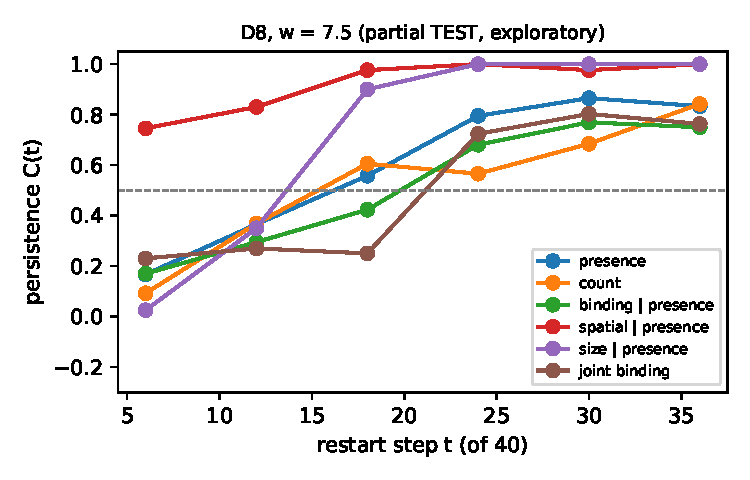
\includegraphics[width=0.75\linewidth]{figures/partial_curves_D8.pdf}
\caption{Chance-corrected persistence $C(t)$ by prompt type under the D8 restart probe ($w=7.5$); dashed line marks $C=0.5$, whose crossing defines $t_{50}$. Partial TEST, exploratory.}\label{fig:partial-curves-D8}
\end{figure}
\begin{figure}[t]\centering
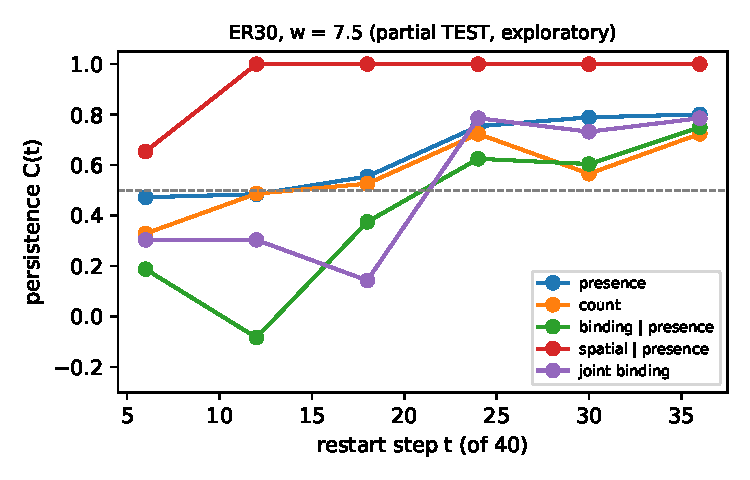
\includegraphics[width=0.75\linewidth]{figures/partial_curves_ER30.pdf}
\caption{Chance-corrected persistence $C(t)$ by prompt type under the ER30 restart probe ($w=7.5$); dashed line marks $C=0.5$. Partial TEST, exploratory.}\label{fig:partial-curves-ER30}
\end{figure}
\begin{figure}[t]\centering
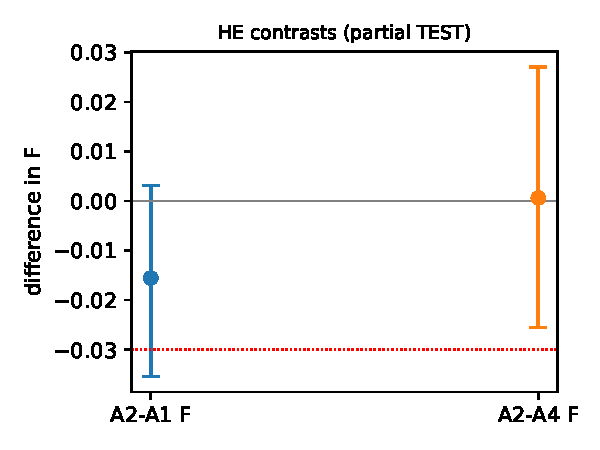
\includegraphics[width=0.75\linewidth]{figures/partial_he.pdf}
\caption{HE contrasts on the composite $F$: A2$-$A1 (90\% CI, non-inferiority; dotted line is the $-0.03$ margin) and A2$-$A4 (95\% CI, timing versus the reversed schedule). Partial TEST, exploratory.}\label{fig:partial-he}
\end{figure}
\begin{figure}[t]\centering
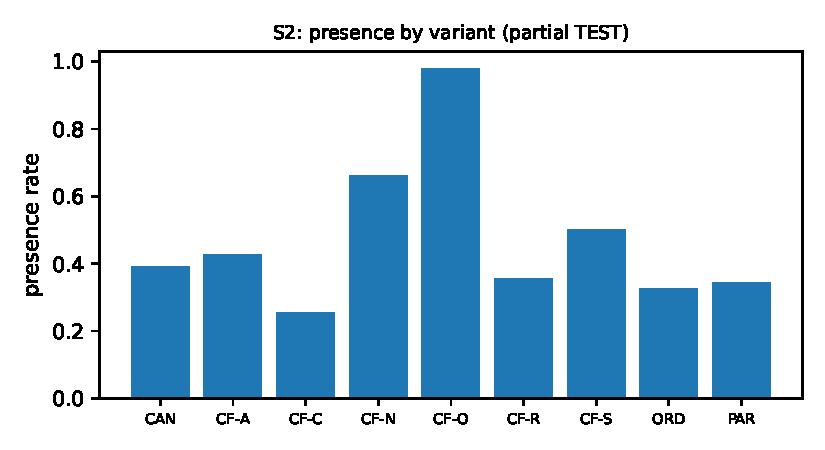
\includegraphics[width=0.75\linewidth]{figures/partial_s2_presence.pdf}
\caption{S2: object-presence rate by prompt variant. Partial TEST, exploratory.}\label{fig:partial-s2-presence}
\end{figure}
\paragraph{Limitations of this analysis.}
\begin{itemize}
\item Missing TEST shards (not imputed): TEST\_CORE shard 2; TEST\_COMMIT shard 2; TEST\_CAG\_SIZE shard 0; estimates cover only the scene groups of the present shards.
\item This is not the registered confirmatory analysis: that requires all nine shards and notebook 04; Holm-adjusted p-values are shown for completeness only.
\item HA is exploratory by its failed DEV precision gate; the full-resample control failed on DEV (Section on DEV results).
\item Only the presence judge met the audit criterion (single annotator, no valid double annotation); count, binding, spatial and size outcomes are exploratory.
\item HE uses only scenes with both A1 and CAG images (67 scenes).
\end{itemize}
